\documentclass[11pt,letterpaper,english]{article}
\usepackage[T1]{fontenc} % Standard package for selecting font encodings
\usepackage{txfonts} % makes spacing between characters space correctly
\usepackage{xcolor} % Driver-independent color extensions for LaTeX and pdfLaTeX.
\usepackage{hyperref}  %The ability to create hyperlinks within the document
%\usepackage{blindtext} % To create text
%\usepackage{mdwlist} % mdwlist for compact enumeration/list items
%\usepackage[pagestyles]{titlesec} % related with sections—namely titles, headers and contents
\usepackage{fancyhdr} % header footer placement

\usepackage[top=1in, bottom=1in, left=1in, right=1in] {geometry} % Margins
\usepackage{graphicx}   % Essential for adding images to you document.

\usepackage{sectsty}
\sectionfont{\large}
\subsectionfont{\normalsize}
\subsubsectionfont{\normalsize \it}

\usepackage[font=bf]{caption}
\captionsetup{labelsep=period}


\pagestyle{fancy} % allows you to use the header and footer commands

\raggedright
\begin{document}

\setlength{\parindent}{0in}% Amount of indentation at the first line of a paragraph.


\pagestyle{fancy} \lhead{Revealing the Physics of Galactic Winds with Petascale GPU Simulations} \rhead{Brant Robertson} \renewcommand{%
\headrulewidth}{0.0pt}




\section{PROJECT PLANS FOR NEXT YEAR} 

The project plans should address the points described below. {\bf This section is typically about 4 pages.} All visual materials, such as charts, graphs, pictures, etc., are included in the page limit; references are {\bf not} included in the page limit.  URLs that provide information related to the application should not be included. \\

Insert paragraph(s).

\subsection{Summarize the Project Plan} 

Briefly explain what advances you expect to accomplish through the next award period and associate these with the overarching goals of your project. Clearly explain the relationships between the milestones, planned production simulations, and expected compute time required for these sets of simulations. Explain any change in the scope of the project (research objectives, computational approach, personnel, etc.) relative to the plans and approach articulated in the original proposal. If resource requirements differ from those of the previous year, provide details on the differences (platform, increased/decreased core-hours, file system and archival storage, networking) and the reasons for them. If you are requesting a new resource, you must provide evidence that your project is optimized to run on that resource. See the ``New Code Applications'' section below. Summarize the requirements that are driving the differences and what science/technology outcomes are expected. Significant changes to the original project scope should be discussed with the INCITE program manager prior to submittal.

Insert paragraph(s).

\subsubsection{Heading 3 (optional)}

Insert paragraph(s).

\subsection{Developmental Work} 

Describe what, if any, developmental work has been carried out and the outcome of this work. Describe what additional development work will be executed, and when. Provide an estimate for the percentage of project time you will spend on developmental computing (e.g., porting, performance analysis) and other nonproduction runs.

Insert paragraph(s).

\subsection{New Code Applications (where relevant)} 

Are you planning to use any new production codes next year that were not included in your original proposal? Or are you proposing use of a new resource not included in your original proposal? If so, provide direct evidence, including supporting quantitative data, for your production application’s parallel performance for the intended research simulations. Ideally, the proposing team will have generated the data. If you cite work by others, explain why it is applicable here. You should use the application code you intend for the production work, not a related code. Data for sample systems not related to the intended research is undesirable. Performance benchmarking should reflect all I/O requirements. Parallel performance data in either strong or weak scaling mode must be provided. Explain how the strong or weak scaling applies to the proposed work. 

NOTE: You may apply for a startup account at one of the centers to conduct performance studies. Applications are available at

ANL: {\href{http://www.alcf.anl.gov/getting-started/apply-for-dd}{http://www.alcf.anl.gov/getting-started/apply-for-dd}}

ORNL: {\href{www.olcf.ornl.gov/support/getting-started/olcf-director-discretion-project-application}{www.olcf.ornl.gov/support/getting-started/olcf-director-discretion-project-application}}

Insert paragraph(s).

If included, call out equations, tables, figures, and references in numerical order in text, such as Eqs. (\ref{Eq. 1}) and (\ref{Eq. 2}), Table \ref{Tab1}, and Fig. \ref{Fig1} below.

\begin{equation} \label{Eq. 1} 
\partial ,\phi +u\cdot \nabla \phi =\nabla ^{2} \phi +\frac{1}{\tau } R\left(\phi \right)\, \, ,
\end{equation} 


\begin{equation} \label{Eq. 2} 
\frac{\partial \phi }{\nabla \phi } =\frac{1}{2} \nabla ^{2} \phi \frac{e^{\frac{-R-R^{2} }{2u} } }{\left(2\tau \right)^{3N/2} } \sqrt{xyz} \, \, \sum 1+23\, \, \, . 
\end{equation} 

\begin{table}[h]
\centering
\caption{Table title}
\label{Tab1}
\begin{tabular}{llll} \\ \hline 
\textbf{Column one} & \textbf{Column two} & \textbf{Column three} & \textbf{Column four} \\ \hline 
 xxx & xxx\textit{${}^{a}$} & xxx & xxx \\ \hline 
xxx & xxx & xxx & xxx \\ \hline 
{\textit{$^{a}$}Footnote here.} \\
\end{tabular}
\end{table}


\begin{figure}
\centering
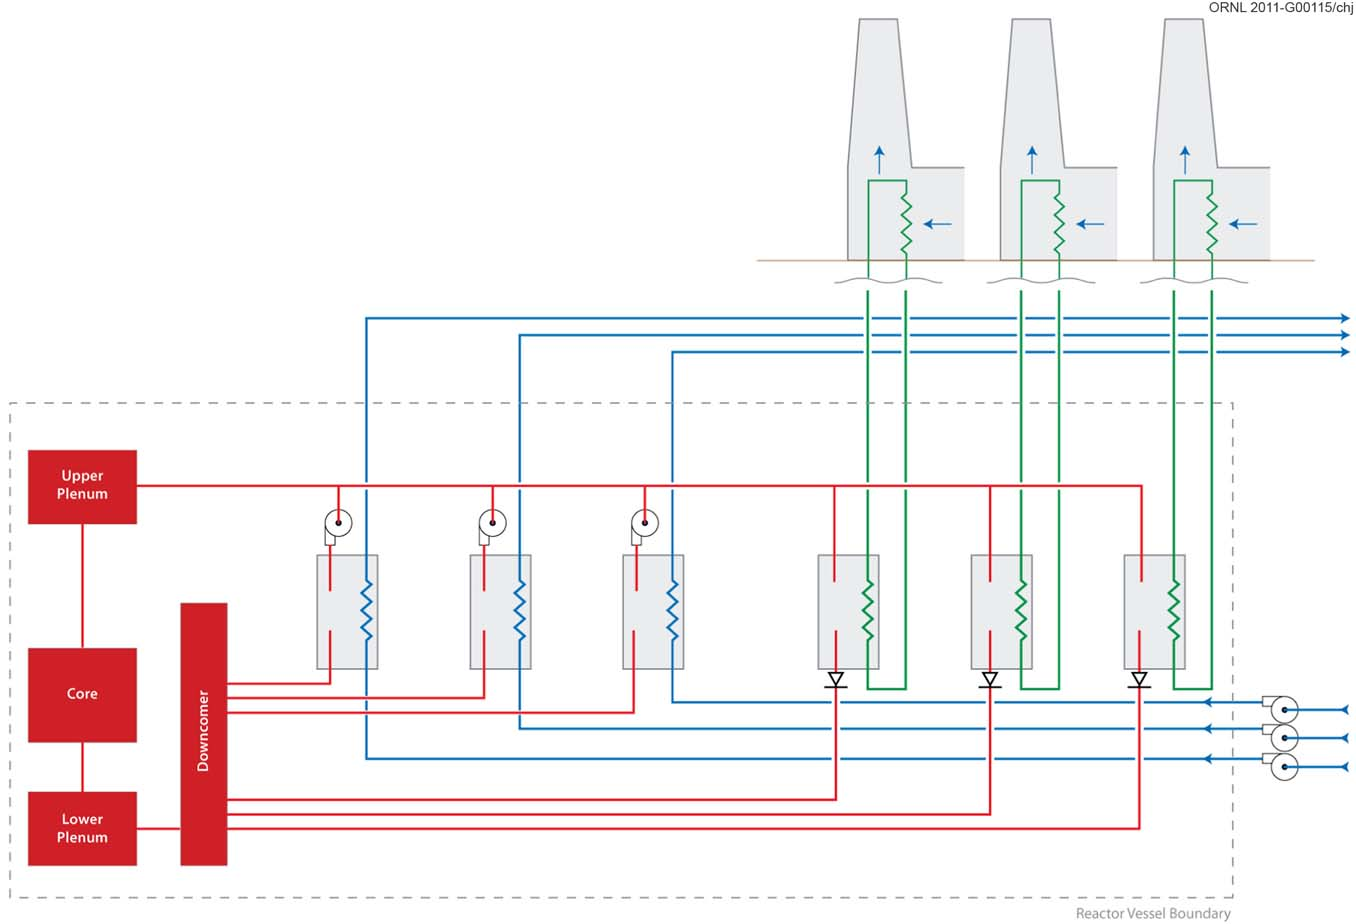
\includegraphics[width=4.52in, height=3.08in, keepaspectratio=true]{image1.jpg}
\caption{Figure caption.}
\label{Fig1}
\end{figure}

\subsubsection{Heading 3 (optional)}

Insert paragraph(s).


\begin{itemize}
\setlength{\itemsep}{-14pt}
\item Text \\ 
\item Text \\
\end{itemize} 
\vspace{-.15in}

\end{document}
